\chapter{Detector Calibration and MC Tuning}
\label{chapter:calibartion}
\thispagestyle{myheadings}
\graphicspath{{4_Chapter_Calibration/Figures/}}

Accurate modeling of physics events and detector response are essential for correct interpretations of KamLAND-ZEN experimental data. This chapter outlines the detector calibration and Monte-Carlo (MC) tuning methods used. Since the commissioning of KamLAND-ZEN 800, no deployed laser or radioactive source calibration was done. This was to avoid any radioactive contamination from inserting these components into the detector. Thus, known backgrounds are the primary tools for detector calibration.
\cite{klz800_arxiv}

\section{Detector Calibration}
The KamLAND detector has taken data for over 20 years. The energy scale, nonlinearity, bias, resolution, and vertex bias and resolutions have been well calibrated and studied. However, it is important to understand the variation of the detector performance over time. Electronics issues, such as HV reduction, channel loss, and detector work can affect our reconstructions. 
\subsection{Variation of Energy Scale Over Time}
As PMT channels are lost or deteriotate into bad channels, or have their gains adjusted, the energy scale of the detector can vary over time. Variation from the beginning of the analysis period in 2019 and until the end of KLZ-800 data-taking in 2024, the energy scale varied by 3\%. 

\begin{figure}[htb]
    \centering
    % Left subplot (A) - Time variation
    \begin{subfigure}[b]{0.48\textwidth}
        \centering
        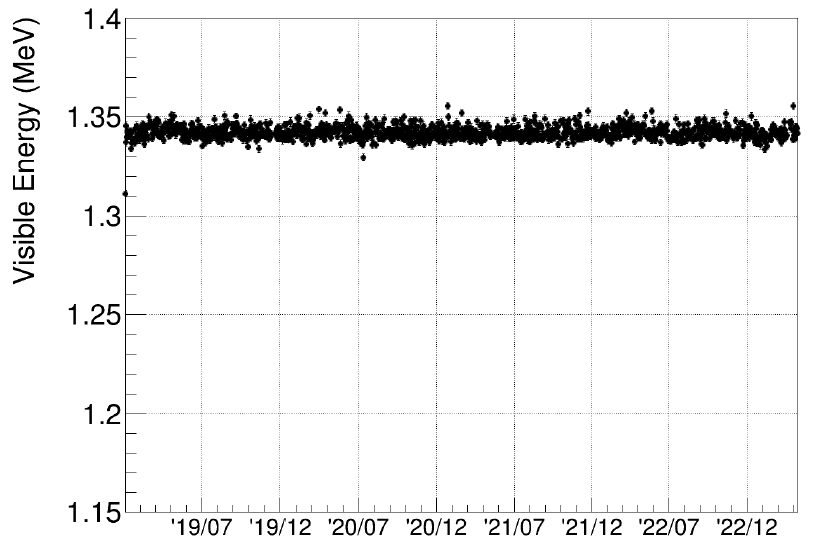
\includegraphics[width=\textwidth]{K40_PEEK_Time.png}
        \caption{Time variation}
        \label{fig:time_variation}
    \end{subfigure}
    \hfill
    % Right subplot (B) - Histogram
    \begin{subfigure}[b]{0.48\textwidth}
        \centering
        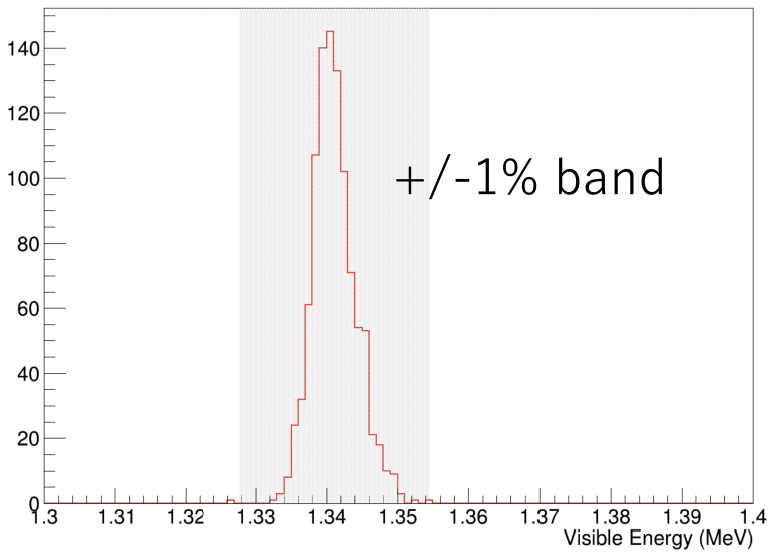
\includegraphics[width=\textwidth]{PEEK_energy.png}
        \caption{Histogram among runs (\%) axis}
        \label{fig:histogram}
    \end{subfigure}
    
    \caption{Time variation of $^{40}$K peak after correction. (A) Time variation of 
    energy scale is corrected using $^{40}$K and this figure is a check using $^{40}$K itself. 
    (B) Fluctuations among runs are within 1\% (gray band).}
    \label{fig:figure51}
\end{figure}
\subsubsection*{$^{40}$K PEEK Gammas}
Reconstructing the $^{40}$K-$\gamma$ peak from balloon PEEK material can help calibrate the energy scale over time. The PEEK material is located 550cm above the center of the detector and is a consistent source of $^{40}$K radioactive decays. The decay energy of the $^{40}$K electron-capture decay to $^{40}$Ar has an energy of $Q_{EC}=1504$ keV. However, as the energy scale of the detector decreases as you move from the center of the detector. This EC-$\gamma$ peak is observed at around $E_{vis}=1.35$ MeV in KamLAND-ZEN. These $^{40}$K PEEK events are selected by the following simple selection:
\begin{itemize}
	\item Passes Flasher Veto
	\item Passes Muon Veto
	\item Passes 2msec veto after muons
	\item cylindrical volume selection around PEEK material ($450<z<600$,$\rho<250$ cm)
\end{itemize}

\subsubsection*{Neutron Capture Gammas}
The KamLAND energy scale is primarily set by neutron captures on Hydrogen. Figure \ref{fig:neutron_capture_energy} shows the variation in neutron capture visible energy over time in XeLS and KamLS. Events are taken simply in a time window following muons. Due to post-muon instability, such as high after-pulsing, PMT ringing, and baseline shifts, the time directly after muons is excluded. An on-off time analysis is performed to subtract any incidental backgrounds and resolve the neutron capture energy distribution.
\begin{itemize}
    \item On-time window : $400<dT<1500 \mu sec$
    \item Off-time window : $2800<dT<4000 \mu sec$
\end{itemize}
\begin{figure}[htb]
	\centering
	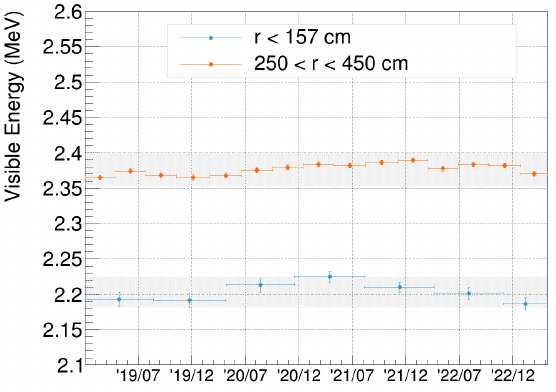
\includegraphics[scale=0.65]{neutron_escale.png}
	\caption{Neutron capture energy over KLZ-800 data-taking. The blue and orange points correspond to XeLS and KamLS respectively. Gray bands show $\pm1\%$ deviation from the average. Note that the energy scale is 7\% higher in KamLS due to the higher scintillator light-yield.}
	\label{fig:neutron_capture_energy}
\end{figure}
\subsubsection*{$2\nu\beta\beta$ Rate}
The tail of the \2nbb decay spectrum is another useful handle on variations in energy scale over time. In the abscence of any XeLS leakage out of the inner balloon, the rate of \2nbb events in an energy range can be used to verify the energy scale. We apply all the \0nbb analysis event selections and a further $1.85<E_{vis}<2.35$ MeV energy selection to select the \2nbb-dominant region. Figure \ref{fig:2nu_stability} shows minor fluctuations, but no clear trend upward or downwards.
\begin{figure}[htb]
	\centering
	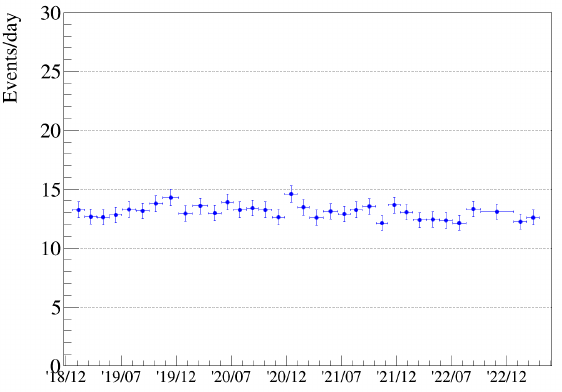
\includegraphics[scale=0.65]{2nu_trend.png}
	\caption{The event rate in the \2nbb dominant energy region over KLZ-800 data-taking.}
	\label{fig:2nu_stability}
\end{figure}
\subsection{MoGURA Stability}
Cosmic ray muon induced spallation reactions are a constant source of well understood background. MoGURA's dead-time-free electronics allow it to observe neutron capture's closer in time to the original muons. This higher tagging efficiency than KAMFEE provides more data that can be used for calibration.

The MoGURA stability performance over time is marked by the neutron capture rate and distributions. Figure \ref{fig:neutron_capture_energy} shows the variation over time of MoGURA's neutron tagging performance. The neutron selection in MoGURA was outline in section \ref{sec:mogura_neutron_reco}.
\begin{figure}[htb]
	\centering
	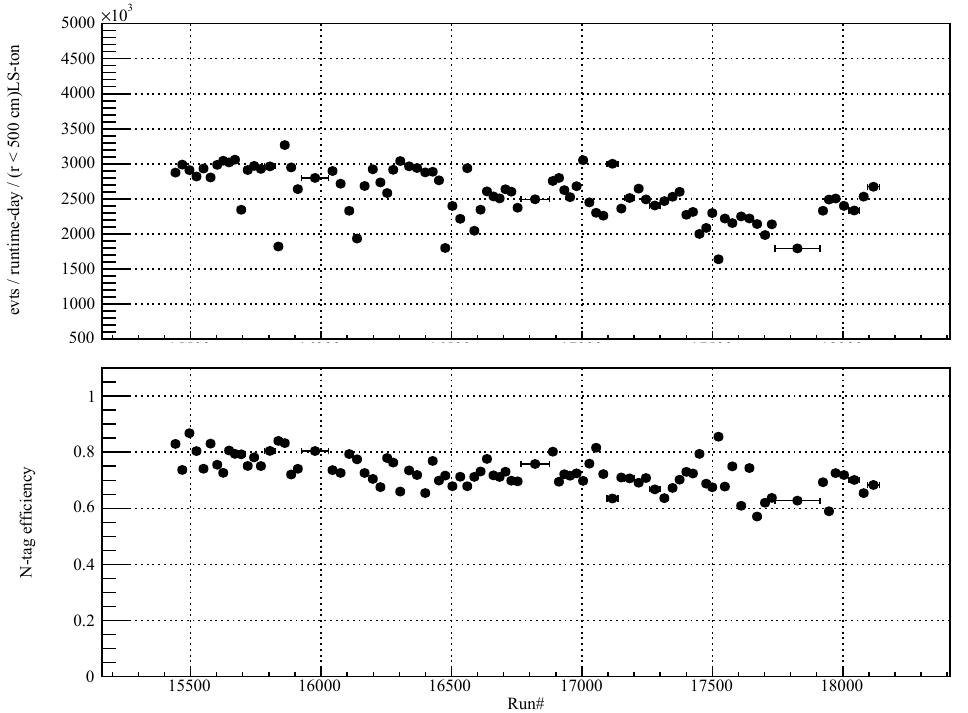
\includegraphics[scale=0.35]{neutron_capture_trend.png}
	\caption{MoGURA's neutron capture rate and neutron tagging efficiency over KLZ-800 data-taking.}
	\label{fig:neutron_capture_trend}
\end{figure}
\subsubsection*{$^{10}$C tagging Stability}
$^{10}$C is an easily isolated, well-understood background that can be further used to monitor detector stability. $^{10}$C tagging via triple coincidence was described in section \ref{sec:mogura_neutron_veto}. Note that for this study, the $^{10}$C selection was adjusted from the \0nbb analysis for higher signal purity.
\begin{itemize}
    \item Select events in KamLS volume $(250<r<400 cm)$ and veto the corrugateed tube $(r>250 cm\& z>0)$
    \item $2.0<E_{vis}<5.0 $ MeV
    \item On-time window: $10<dT<90$ sec
    \item Off-time window: $300<dT<1000$ sec
\end{itemize}
The on-time window begins at 10 seconds to exclude the $^{6}$He spallation background with a 1.16 second lifetime and $Q_\beta=3.5$ MeV. Figure \ref{fig:c10_mogura} shows the characteristic distributions that identify the dataset as $^{10}$C. The rate is estimated by fitting an exponential plus constant background to the $dT$ distribution. The $dR$, distance to nearest neutron, distribution is modeled by an $exGaussian$, exponentially modified Gaussian. The variation in $^{10}$C rate and mean of the exGaussian function are shown in Figure \ref{fig:C10_stability}
\begin{figure}[htb]
	\centering
	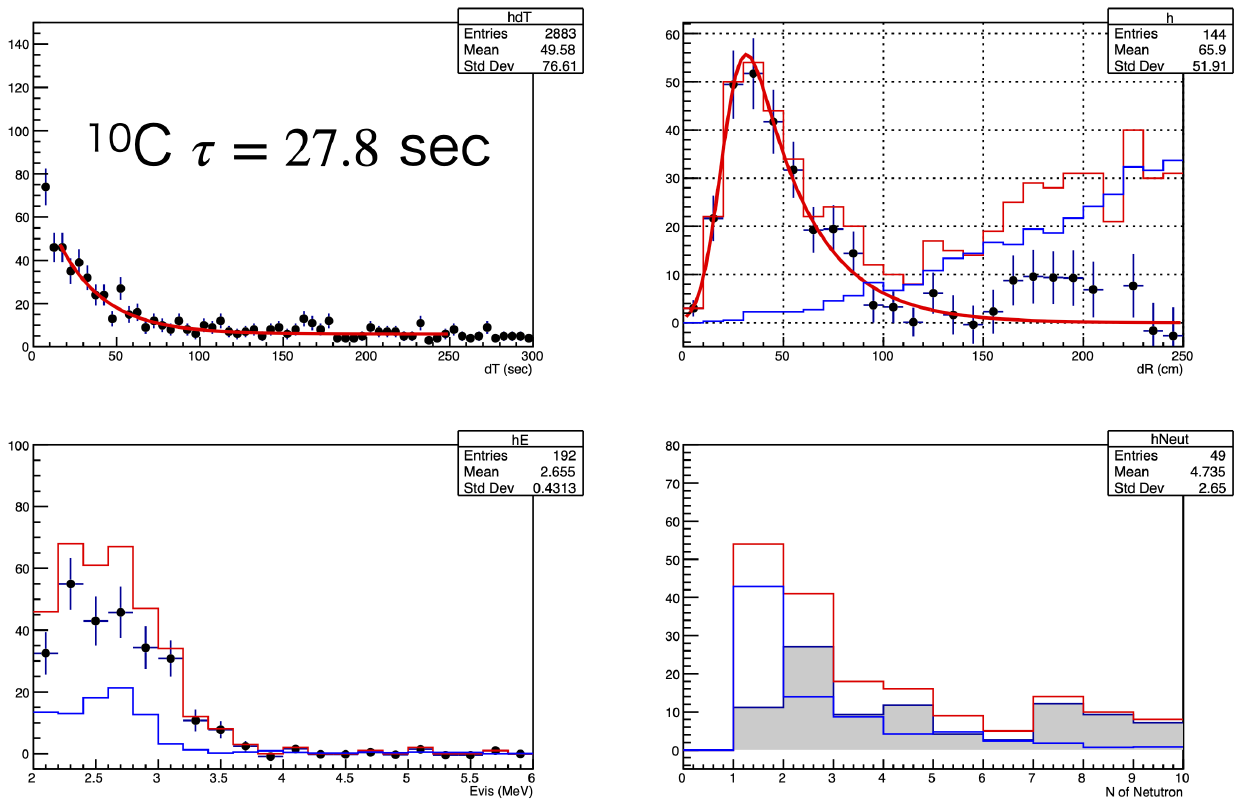
\includegraphics[scale=0.35]{mogura_c10.png}
	\caption{Characteristic distributions of $^{10}$C decays. Red and blue histograms show on-time and off-time events respectively, and the black markers or grey histograms show the subtracted distributions (on-time - off-time). }
	\label{fig:c10_mogura}
\end{figure}

\begin{figure}[htb]
    \centering
    \begin{subfigure}[b]{0.48\textwidth}
        \centering
        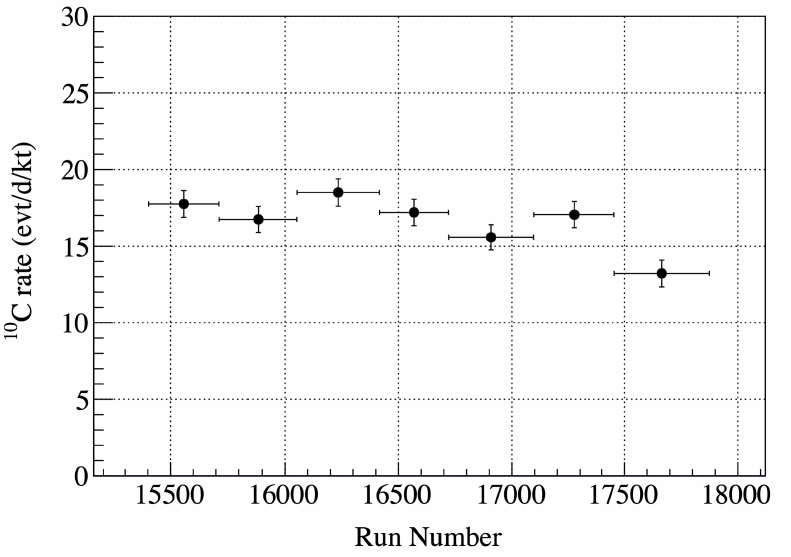
\includegraphics[width=\textwidth]{c10_rate.png}
    \end{subfigure}
    \hfill
    \begin{subfigure}[b]{0.48\textwidth}
        \centering
        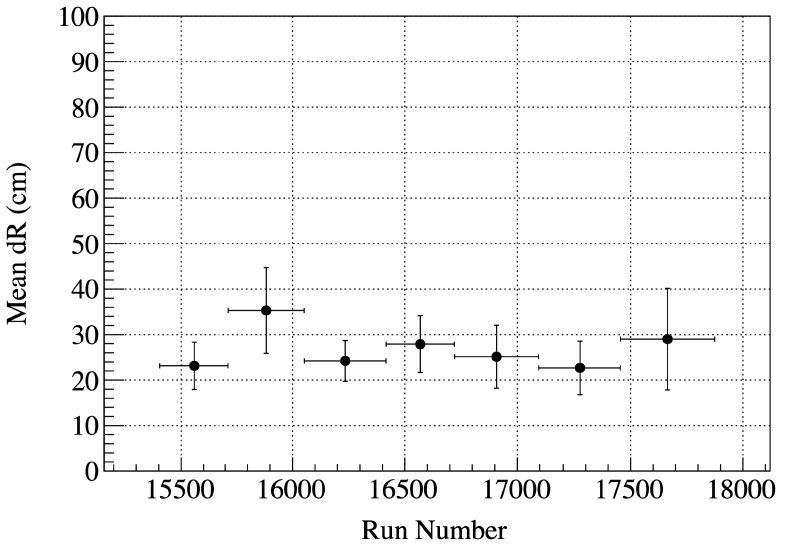
\includegraphics[width=\textwidth]{c10_dist.png}
    \end{subfigure}
    
    \caption{Time variation of $^{10}$C rate and dR distribution shape over KLZ-800 data-taking.}
    \label{fig:C10_stability}
\end{figure}

\section{MC Tuning}
KamLAND physics simulation is built on two simulation tools: GEANT4 and FLUKA. GEANT4 is used to simulate the distributions of signals, backgrounds decays, and scintillation light propagation in KamLAND detector media. KamLAND's GEANT4-based simulation tool chain is called KLG4Sim. FLUKA is used to simulate cosmic-ray muon induced spallation. Namely for neutron multiplicity and topology and spallation isotope production. 
\subsection{Geant4 (KLG4)}
KLG4 simulations used in this thesis analysis were tuned in \cite{ozaki_phd} and \cite{takeuchi_phd}. This section describes their prior work in tuning KLG4 parameters.
\subsubsection*{KamLS Tuning}
KamLS properties, the outer scintillator volume without dissolved xenon, are tuned using source calibration data taken on January 16, 2018. The calibartion deployment involved moving a composite radioactive soure between -550 and 550 cm in 50cm intervals. With 20 minutes of data-taking at each position. Table \ref{tab:calib_soure} describes the source composition.

\begin{table}[h]
\centering
\caption{Summary of radioactive source. Estimated intensities are as of January 17, 2018 on which the calibration DAQ was taken.}
\label{tab:calib_soure}
\begin{tabular}{lccc}
\hline
Construction date & \multicolumn{3}{c}{Aug. 24, 2015} \\
DAQ date & \multicolumn{3}{c}{Jan. 16, 2018} \\
Source ID & \multicolumn{3}{c}{Kam-41 (composite source)} \\
\hline
 & $^{137}$Cs & $^{68}$Ge & $^{60}$Co \\
Particle & 1$\gamma$ & 2$\gamma$ & 2$\gamma$ \\
Energy (keV) & 661.7 & 511.0 & 1173.2, 1332.5 \\
Initial Intensity (Bq) & 181 & 419 & 322 \\
Estimated Intensity (Bq) & 180 & 356 & 234 \\
\hline
\end{tabular}
\end{table}
Figure \ref{fig:calib_source} shows the $N_{hit}$ and total charge spectra of the composite source, with clearly visible gamma peaks. The gamma peaks are used to calibrate the nonlinearity of KamLS energy scale. The figure also shows the tuned KLG4 spectra that agrees well with data after tuning.

The energy scale is also tracked through position, via calibration source deployment. The deployment data was used to tune material properties like attenuation length, re-emission probabilities, and scattering probabilities. Figure \ref{fig:calib_source_pos} shows the position dependence of total charge for each source isotope. The variability and simulation reproducibility with tuning is deteriorates as we move from the center of the detector. The physics analysis presented in this thesis focuses on data within 250cm. In this region, the deviation is within 2\%.
\begin{figure}[htb]
    \centering
    \begin{subfigure}[b]{0.48\textwidth}
        \centering
        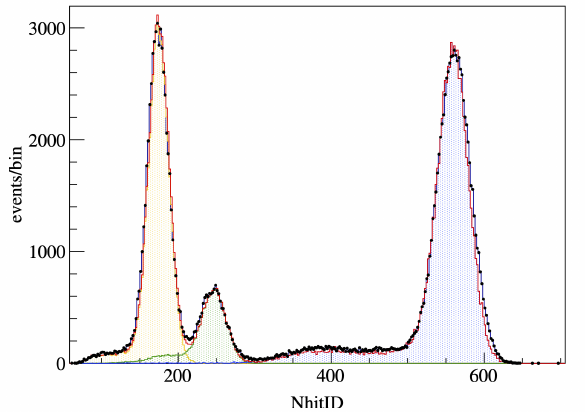
\includegraphics[width=\textwidth]{calib_source_nhit.png}
    \end{subfigure}
    \hfill
    \begin{subfigure}[b]{0.48\textwidth}
        \centering
        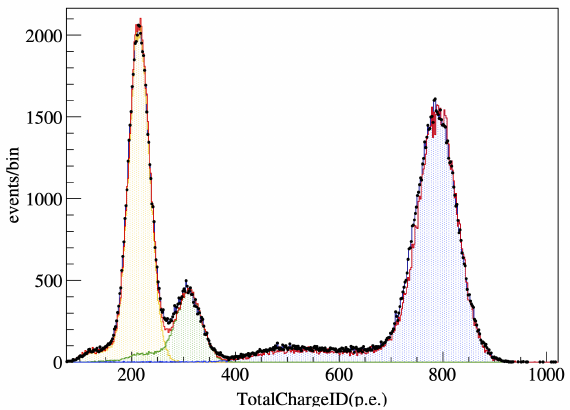
\includegraphics[width=\textwidth]{calib_source_charge.png}
    \end{subfigure}
    
    \caption{$N_{hit}$ and total charge distribution of source calibration. Black plots show data and colored histograms (orange: 137 Cs, green: 68Ge, blue: 60 Co) show MC simulation. MC spectra are well tuned to data in both $N_{hit}$ and total charge. Figures from \cite{ozaki_phd}}
    \label{fig:calib_source}
\end{figure}

\begin{figure}[htb]
	\centering
	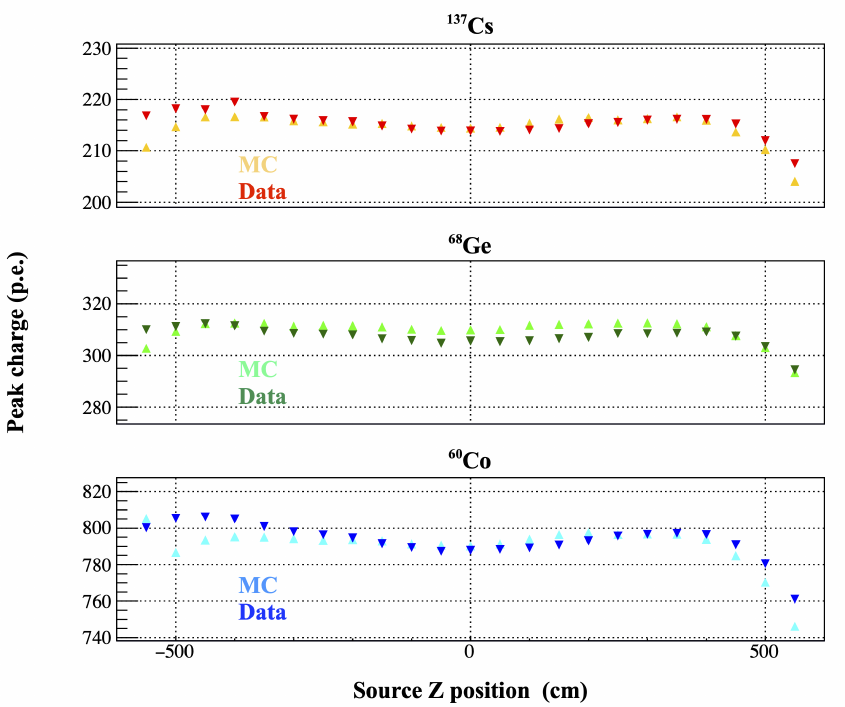
\includegraphics[scale=0.35]{calib_source_pos.png}
	\caption{Position dependence of total charge peak for each calibration source isotope \cite{ozaki_phd}}
	\label{fig:calib_source_pos}
\end{figure}

\subsubsection*{XeLS Tuning}
There are no source calibration located in XeLS. Alternatively, some background sources are available to calibrate the detector. $^{222}$Rn is mixed in XeLS by emanation from pipeline or buffer tanks during xenon resolving work. A sequential decay of daughter isotopes $^{214}$Bi-Po can be tagged using delayed coincidence and they exists only in XeLS. The half life of $^{222}$Rn is 3.8 days and after completion of xenon resolving work, $^{222}$Rn does not supplied. Thus $^{214}$Bi-Po as high statistic calibration source is available only in first several months of KamLAND-Zen 800 observation. Birk's constant, attenuation length, scattering probability, LS time properties, and re-emission for XeLS are tuned using $^{214}$Bi-Po.

\subsubsection*{Position-dependent Energy Correction}

Position dependence, over radius and $\theta$, of visible energy in XeLS is observed using the $^{214}$Po $alpha$ decay peak. The deviation from the center of the detector is reproduced in KLG4 as shown in Figure \ref{fig:po214_alpha}. The MC correction factors were tuned to ensure that the MC \0nbb decay peak in XeLS does not have a position dependence.

\begin{figure}[htb]
\centering
\begin{subfigure}[b]{0.45\textwidth}
    \centering
    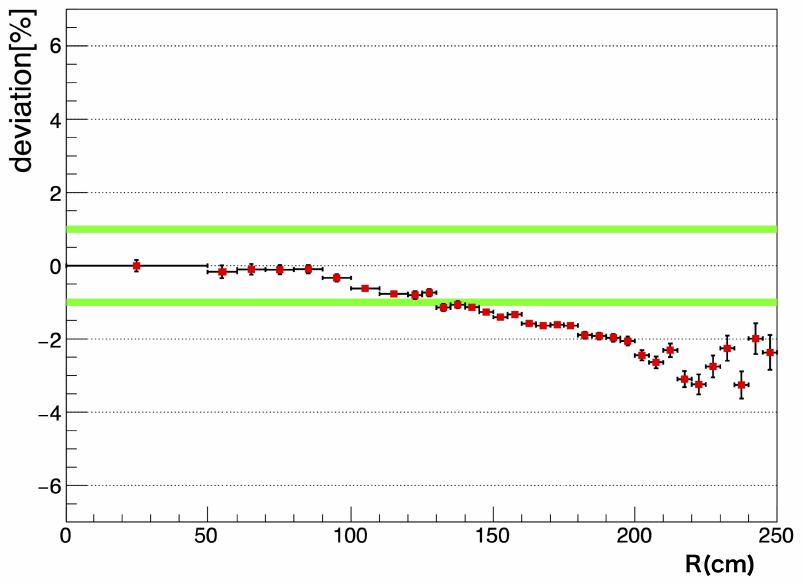
\includegraphics[width=\textwidth]{po214_data.png}
    \caption{Data}
    \label{fig:po214_data}
\end{subfigure}
\hfill
\begin{subfigure}[b]{0.45\textwidth}
    \centering
    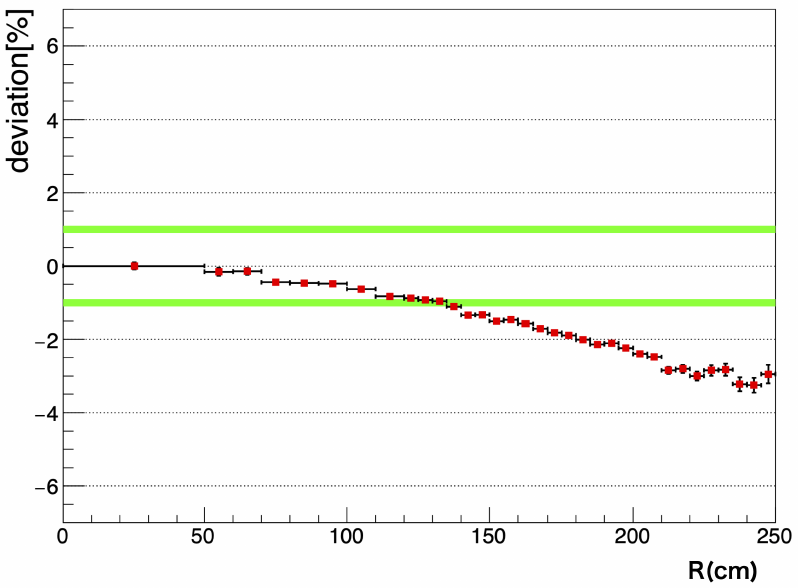
\includegraphics[width=\textwidth]{po214_mc.png}
    \caption{MC (before correction)}
    \label{fig:po214_mc_before}
\end{subfigure}

\vspace{1cm}

\begin{subfigure}[b]{0.45\textwidth}
    \centering
    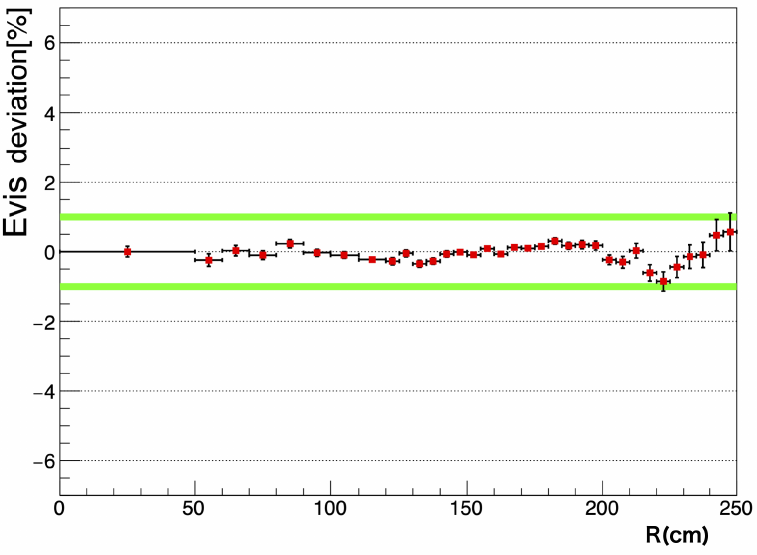
\includegraphics[width=\textwidth]{po214_mc_corr.png}
    \caption{MC (after correction)}
    \label{fig:po214_mc_after}
\end{subfigure}

\caption{Radius dependence of total charge of $^{214}$Po. Figures from \cite{ozaki_phd}.}
\label{fig:po214_alpha}
\end{figure}

\subsubsection*{Energy Non-Linearity}
The visible energy and the energy deposited by charged particles have a nonlinear relation due to the scintillation quenching and the contribution of Cherenkov light. The following model is well known as Birks formula:
\begin{equation}
    \label{eq:birks_law}
    \frac{dL}{dx}\propto\frac{dE/dx}{1+kB\cdot dE/dx^\prime}
\end{equation}
where $dL/dx$ is light yield per unit length along particle track, $dE/dx$ is energy deposited per unit length, and $kB$ is the Birks' constant which is material dependent. Charged particles also emit cherenkov light, the proportion of the light yield attributed to cherenkov radiation is denoted by the chrenkov-scintillation ratio, $R$. Tagged $^{214}$Bi data is used to tune $kB$ and $R$. The tagged $^{214}$Bi data in XeLS is primarily from the early $^{222}$Rn-rich period. The tuning analysis was performed in \cite{ozaki_phd} and \cite{takeuchi_phd}. Figure \ref{fig:kb_r_chisquare} shows a $\Delta\chi^2$ scan over $kB$ and $R$ and the best fit of $(kB, R)=(0.31, 0.01)$. These are the values used in KLG4 for background and signal simulation. Figure \ref{fig:bipo_tune} shows the result of XeLS tuning. The BiPo decay energies are matched to data and the spatial correlation between the coincident decays agree.

\begin{figure}[htb]
	\centering
	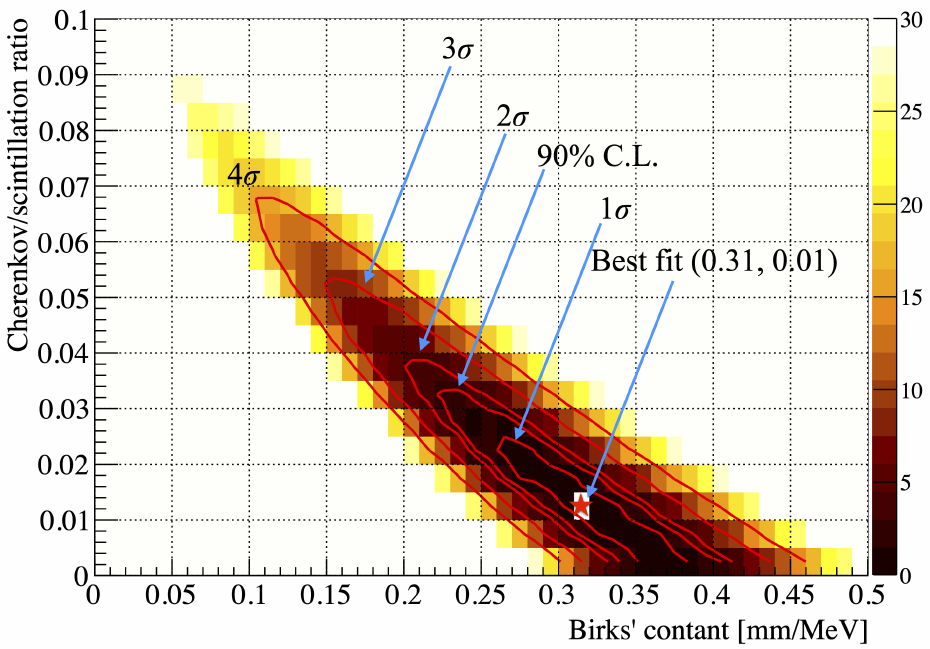
\includegraphics[scale=0.35]{kb_r_chisquare.png}
	\caption{$\Delta\chi^2$ scan over $kB$ and $R$}
	\label{fig:kb_r_chisquare}
\end{figure}

\begin{figure}[htb]
    \centering
    \begin{subfigure}[b]{0.48\textwidth}
        \centering
        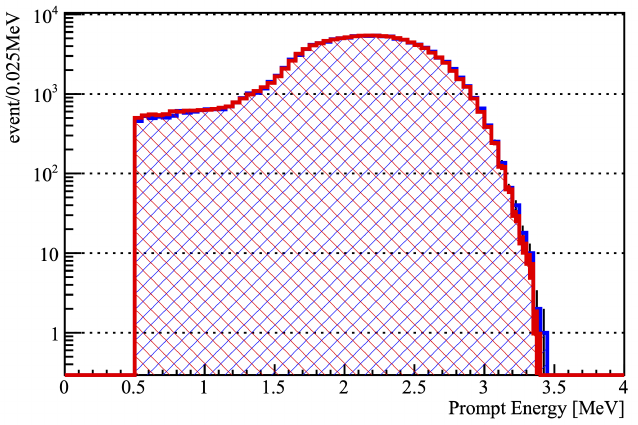
\includegraphics[width=\textwidth]{bi214_spec_tune.png}
    \end{subfigure}
    \hfill
    \begin{subfigure}[b]{0.48\textwidth}
        \centering
        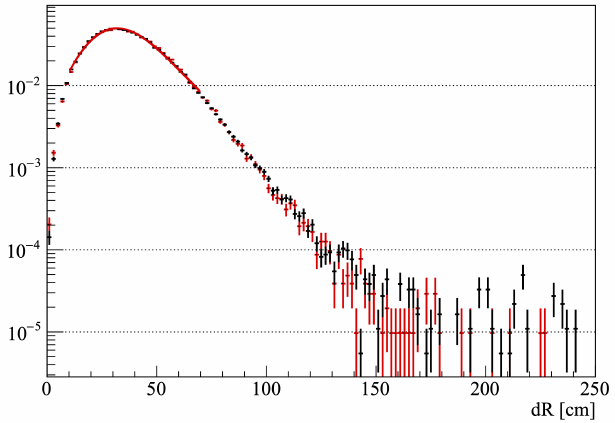
\includegraphics[width=\textwidth]{bipo_dR.png}
    \end{subfigure}
    
    \caption{Tuned $^{214}$Bi-$\beta$ decay energy spectrum and spatial correlation of delayed-coincidence Bi-Po decays. Figures from \cite{takeuchi_phd}}
    \label{fig:bipo_tune}
\end{figure}
\subsubsection*{Energy Scale}
The overall energy scale of KamLS and XeLS are tuned by the neutron capture gamma peak of 2.2 MeV. XeLS introduces extra quenching by the xenon which reduces the light yield in XeLS slightly. Figure \ref{fig:neutron_capture_energy} shows the peak energies used. This is the same dataset used for the energy scale time variation check.
\subsection{FLUKA}
FLUKA simulation software is used to predict cosmic muon spallation isotope yields and neutron production. The FLUKA version used in this modeling is FLUKA 2011.08.patch. Simulations and the results are described in \cite{klz_zenon_spallation}.
\subsubsection*{Simulation Configuration}

\subsubsection*{Radioactive Decays}
\subsubsection*{Tuning With $^{10}$C}

